
\documentclass[12pt]{article}

\usepackage{Homework}

% Creates the header and footer.
\pagestyle{fancy}
\fancyhead[l]{Michael Hoon, $1006617$}
\fancyhead[c]{40.017 Probability \& Statistics HW1}
\fancyhead[r]{\today}
\fancyfoot[c]{\thepage}
\renewcommand{\headrulewidth}{0.2pt} %Creates a horizontal line underneath the header
\renewcommand{\footrulewidth}{0.2pt}
\setlength{\headheight}{15pt} %Sets enough space for the header
\newcommand{\HRule}[1]{\rule{\linewidth}{#1}}


\begin{document}

% \title{Another fancyhdr demo}
% \author{\texttt{tex.stackexchange} \textit{et al}}
% \maketitle
% \newpage


\title{ \normalsize \textsc{} 
        \\ [2.0cm]
		\HRule{1.5pt} \\
		\LARGE \textbf{\uppercase{40.017 Probability \& Statistics} 
        \HRule{2.0pt} \\ [0.6cm]
        \LARGE{Homework 1} \vspace*{10\baselineskip}}
		}
\date{\today}
\author{\textbf{Michael Hoon} \\ 1006617}

\maketitle 
\newpage


\section*{Question 1}
\subsection*{(a)}
Let $A$ be the random variable denoting the number of questions chosen from section A. Since the student 'samples' the question without replacement, $A$ follows a hypergeometric distribution $A \sim \text{hypgeo}(12,9,9)$. The pmf $f(x)$ is given by:

\begin{equation*}
    f(x) = \mathbb{P}(X = x) = \frac{\binom{j}{x}{\binom{k}{n-x}}}{\binom{j+k}{n}}
\end{equation*} \\ 

\noindent for 6 questions from section A, we have $\mathbb{P}(X=6)$:

\begin{align*}
    \mathbb{P}(X=6) &= \frac{\binom{9}{6}\binom{9}{6}}{\binom{18}{12}} \\ 
    &= 0.380090 \\
    &\boxed{\approx 0.380}
\end{align*}

\subsection*{(b)}
Now we need to consider two cases, one where 5 questions come from Section A and the other 7 from Section B, and vice versa. i.e. 

\begin{align*}
    \mathbb{P}(A = 5) + \mathbb{P}(A = 7) &= \frac{\binom{9}{5}\binom{9}{7}}{\binom{18}{12}} + \frac{\binom{9}{7}\binom{9}{5}}{\binom{18}{12}} \\ 
    &= 0.4886877 \\ 
    &\boxed{\approx 0.489}
\end{align*}

\newpage

\section*{Question 2}

\subsection*{(a)}

To find the probability that at least 1 man receives his own hat, we consider the complementary case of no man receiving his own hat, given by $D_6$. Thus:

\begin{align*}
    \mathbb{P}(\text{'at least 1 man receives his own hat'}) &= 1 - \frac{D_{6}}{6!} \\ 
    &= 1 - \frac{6! (1-\frac{1}{1!}+\frac{1}{2!}- \frac{1}{3!}+\frac{1}{4!} - \frac{1}{5!}+\frac{1}{6!})}{6!} \\
    &= \boxed{\frac{91}{144}}
\end{align*}

\subsection*{(b)}

Again we consider the complementary case that no man receives his own hat, or only 1 man receives his own hat. Thus:

\begin{align*}
    \mathbb{P}(\text{'at least 2 men receives their own hats'}) &= 1 - \underbrace{\frac{D_{6}}{6!}}_{\substack{\text{no man receives} \\ \text{their own hat}}} - \underbrace{\frac{6 \times D_{5}}{6!}}_{\substack{\text{1 man receives} \\ \text{his own hat}}} \\ 
    &= \frac{91}{144} - 6 \times \frac{5!(1-\frac{1}{1!}+\frac{1}{2!}-\frac{1}{3!}+\frac{1}{4!}-\frac{1}{5!})}{6!}\\
    &= \boxed{\frac{191}{720}}
\end{align*}

\subsection*{(c)}

The probability that at least 5 men receive their own hats can be interpreted as every man receiving their own hats, since if 5 men receive their own hats, the last man will automatically also receive his own hat. There is only 1 way for all 6 men to receive their own hats, so we have:


\begin{align*}
    \mathbb{P}(\text{'at least 5 men receives their own hats'}) &= \frac{1}{6!} \\ 
    &= \boxed{\frac{1}{720}}
\end{align*}

\newpage 

\section*{Question 3}

\subsection*{(a)}
Since $X$ is the number of coin tosses upon completion, we model $X$ as a geometric distribution with the "success" being obtaining a $\mathtt{T}$: $X \sim \text{geometric}(\frac{1}{2})$, $X \in \{1,2,\dots,n\}$. For $x\in \{1, 2, \dots, n-1\}$, we thus have: $\mathbb{P}(X = x) = (1-\frac{1}{2})^{x-1}(\frac{1}{2}) = (\frac{1}{2})^{x}$. As for $x = n$, we take the complement of all the other probabilities (since they sum to 1):

\begin{align*}
    \mathbb{P}(X = n) &= 1 - \left(\sum_{i=1}^{n-1} \mathbb{P}(X = i)\right) \\ 
    &= 1 - \left( \sum_{i=1}^{n-1} \left(\frac{1}{2}\right)^{i} \right) \\ 
    &= 1 - \frac{\frac{1}{2}(1 - (\frac{1}{2})^{n-1-1+1})}{1- \frac{1}{2}} \\ 
    &= \left(\frac{1}{2}\right)^{n-1}
\end{align*}


\noindent The p.m.f. table is shown below: \\ 

\begin{center}
    \begin{tabular}{|c | c | c | c | c | c |}
       \hline 
       x & 1 & 2 & 3 & \dots & n \\ \hline 
       $\mathbb{P}(X = x)$ & $\frac{1}{2}$ & $(\frac{1}{2})(\frac{1}{2})$ & $(\frac{1}{2})(\frac{1}{2})(\frac{1}{2})$ & \dots & $(\frac{1}{2})^{n-1}$ \\ \hline
    \end{tabular}
\end{center} 

\noindent and in piecewise notation: 

\begin{equation*}
    \boxed{\mathbb{P}(X = x) = \begin{cases}
        \left(\displaystyle\frac{1}{2}\right)^{x}, \qquad x \in \{1, 2, \dots , n-1\} \\ 
        \left(\displaystyle\frac{1}{2}\right)^{x-1}, \quad x = n
    \end{cases}}
\end{equation*}


\subsection*{(b)}
To find $ \mathbb{E}(X)$, we sum over both cases of the p.m.f:

\begin{align}
    \mathbb{E}(X) &= \sum_{i=1}^{n-1} i \cdot \mathbb{P}(X = i) + n \cdot \left(\frac{1}{2}\right)^{n-1} \\ \nonumber
    &= \sum_{i=1}^{n-1} i \cdot \left(\frac{1}{2}\right)^{i} + n \cdot \left(\frac{1}{2}\right)^{n-1} \\ \nonumber
    &= \frac{1}{2 }\sum_{i=1}^{n-1} i \cdot \left(\frac{1}{2}\right)^{i-1} + n \cdot \left(\frac{1}{2}\right)^{n-1} \\ \nonumber
\end{align}

\noindent Using the hint, we differentiate the finite geometric series from the fact that $\frac{d}{dx} x^{a} = ax^{a-1}$. Letting $r = \frac{1}{2}$: 

\begin{align*}
    \frac{\text{d}}{\text{d}r} \left[\sum_{i=0}^{n-1} r^{i} \right] &= \frac{\text{d}}{\text{d}r} \left[\frac{1 - r^{n}}{1-r} \right]\\ 
    \sum_{i=1}^{n-1} i \cdot r ^{i-1} &= \frac{1-r^{n}}{(1-r)^{2}} - \frac{nr^{n-1}}{1-r} \\ 
\end{align*}

\noindent Now, substituting back into Equation (1), we have:

\begin{align*}
    \mathbb{E}(X) &= \frac{1}{2} \left[ \frac{1 - (\frac{1}{2})^{n}}{(1-\frac{1}{2})^{2}} - \frac{n(\frac{1}{2})^{n-1}}{1-\frac{1}{2}}\right] + n \cdot \left(\frac{1}{2}\right)^{n-1} \\ 
    &= \frac{1}{2} \left[4\left(1-\left(\frac{1}{2}\right)^{n}\right)-2n\left(\frac{1}{2}\right)^{n-1}\right] + n \cdot \left(\frac{1}{2}\right)^{n-1} \\
    &= 2- \left(\frac{1}{2}\right)^{n-1} - n\cdot\left(\frac{1}{2}\right)^{n-1} + n \cdot \left(\frac{1}{2}\right)^{n-1} \\
    &=  \boxed{2- \left(\frac{1}{2}\right)^{n-1}}
\end{align*}

\newpage

\section*{Question 4}
Chebyshev's inequality in the standard form gives the \textbf{upper bound} for the probability of being $k$ standard deviations $(\sigma = 5)$ away from the mean $\mu = 50$. 

\begin{equation}
    \mathbb{P}(|X - \mu| \geq k\sigma) \leq \frac{1}{k^{2}}
\end{equation} \\ 

\noindent Let $X$ be the weekly production of the factory (in tons). We want to find the probability $ \mathbb{P}(41 \leq X \leq 61)$. Since the bounds are not symmetric about $\mu$, we need the tighter bound $ \mathbb{P}(41 \leq X \leq 59)$. Then, the value of $k$ is now $k = \frac{9}{5}$ standard deviations away from the mean. \\ 

\noindent Graphically, we can see that \\

\begin{figure}[H]
    \centering
        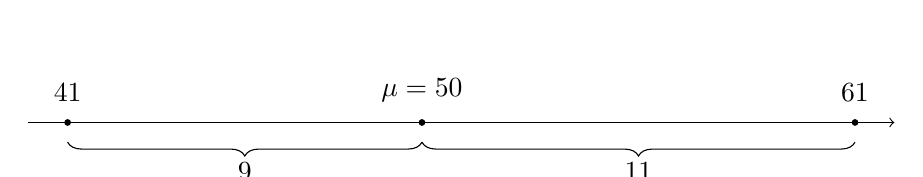
\begin{tikzpicture}[scale=0.5]
            % Draw number line
            \draw[->] (40,0) -- (62,0);
            
            % Draw points
            \foreach \x/\label in {41/41, 50/\(\mu = 50\), 61/61}
            \filldraw (\x,0) circle (2pt) node[above=4pt] {\label};
            
            % Draw underbraces
            \draw[decorate,decoration={brace,amplitude=5pt,mirror}] (41,-0.5) -- (50,-0.5) node[midway,below=4pt] {9};
            \draw[decorate,decoration={brace,amplitude=5pt,mirror}] (50,-0.5) -- (61,-0.5) node[midway,below=4pt] {11};
        \end{tikzpicture}
    \caption{Illustration of bounds}
    \label{fig:4-ineq}
\end{figure}

\noindent From Equation (2), to find a \textit{lower} bound, we need to take the complement:

\begin{equation}
    \mathbb{P}(|X - \mu| < k\sigma) \geq 1 - \frac{1}{k^{2}}
\end{equation} \\ 

\noindent Thus the lower bound for the probability that the weekly production is between 41 and 61 tons is: 

\begin{align*}
    \mathbb{P}(41 \leq X \leq 61) &\geq \mathbb{P}\left(|X - \mu| < \frac{9}{5}\sigma\right) \\ 
    &\geq 1 - \frac{1}{\left(\frac{9}{5}\right)^{2}} \\ 
    &= \boxed{\frac{56}{81}}
\end{align*}

\newpage

\section*{Question 5}

Let $X \sim \text{negbin}(n,p)$. In the recitation, to find the MGF of $X$, since the negative binomial distribution is the sum of $n$ independent geometric distributions, let $Y \sim \text{Geometric}(p)$, and $q = 1-p$.

\begin{equation}
    M_Y (t) = \frac{p e^{t}}{1- qe^{t}}
\end{equation} \\ 

\noindent We have $Y_{1} + Y_{2} + \dots + Y_n \sim \text{negbin}(n,p)$. Since each $Y_i$'s are independent, by the sum property, the MGF of $X$ is given by: 

\begin{align*}
    M_{Y_{1} + Y_{2} + \dots + Y_n} (t) &= M_{Y_{1}} (t) \cdot M_{Y_{2}} (t) \dots M_{Y_n}  (t) \\ 
    &= \left[M_Y(t)\right]^{n} \\ 
    &= M_X (t) \\ 
    &= \left[\frac{p e^{t}}{1- qe^{t}} \right] ^{n}
\end{align*} 

\begin{proof} 
    To find $ \mathbb{E}(X)$, we need to find the first moment, which requires the derivative:

    \begin{align*}
        M_X (t) &= \left[\frac{p e^{t}}{1- qe^{t}} \right] ^{n} \\ 
        M'_X (t) &= n \left[ \frac{p e^{t}}{1-qe^{t}}\right]^{n-1} \cdot  \frac{\text{d}}{\text{d}t} \left[ \frac{pe^{t}}{1-qe^{t}}\right] \\ 
        &= n \left[ \frac{p e^{t}}{1-qe^{t}}\right]^{n-1} \cdot \left[ \frac{pe^{t}(qe^{t} + (1-qe^{t}))}{(1-qe^{t})^{2}}\right] \\ 
        &= n \left[ \frac{p e^{t}}{1-qe^{t}}\right]^{n-1} \cdot \left[ \frac{pe^{t}}{(1-qe^{t})^{2}}\right] \\ 
        &= \left[ \frac{pe^{t}}{1-qe^{t}}\right] \cdot \frac{n}{(1-qe^{t})} \\
    \end{align*}

    \noindent Now, to find $\mathbb{E}(X)$, we set $t = 0$:

    \begin{align*}
        M'_X (0) &= \left[ \frac{p}{1-q}\right]^{n} \cdot \frac{n}{1-q} \\ 
        &= \left[ \frac{p}{1-(1-p)}\right]^{n} \cdot \frac{n}{1- (1-p)} \\ 
        &= \boxed{\frac{n}{p}} = \mathbb{E}(X)
    \end{align*}
\end{proof}


\section*{Question 6}
\subsection*{(a)}
To find the MGF of $X$, since $X$ is continuous, we need to integrate over all $X$, taking note that the MGF is only defined on $-1 <t<1$: 

\begin{align*}
    M_X (t) &= \int_{-\infty}^{\infty} e^{tx}f(x) \, \mathrm{d}x \\ 
    &= \int_{-\infty}^{\infty} e^{tx}\frac{1}{2}e^{-|x|} \, \mathrm{d}x \\ 
    &= \int_{-\infty}^{0} e^{tx} \cdot \frac{1}{2} e^{x} \, \mathrm{d}x + \int_{0}^{\infty} e^{tx} \cdot \frac{1}{2} e^{-x} \\
    &= \frac{1}{2}\left[ \int_{-\infty}^{0} e^{(t+1)x} \, \mathrm{d} x+ \int_{0}^{\infty} e^{(t-1)x} \, \mathrm{d} x\right] \\ 
    &= \frac{1}{2} \left[ \frac{1}{t+1} e^{(t+1)x} \Biggr|_{-\infty}^{0} + \frac{1}{t-1} e^{(t-1)x} \Biggr|_{0}^{\infty}\right] \\ 
    &= \frac{1}{2}\left[\frac{1}{t+1} - \frac{1}{t-1}\right] \qquad \because (-1 < t < 1) \\
    &= \frac{1}{2} \left[ \frac{t-1-t-1}{(t+1)(t-1)}\right] \\ 
    &= \frac{1}{2} \left[ \frac{-2}{t^{2} - 1}\right] \\ 
    &= \boxed{\frac{1}{1-t^{2}}}
\end{align*}

\subsection*{(b)}

Note that $\text{Var}(X) = \mathbb{E}(X^{2}) - \mathbb{E}(X)^{2}$, so we need to find the first and second moments. For the first moment we need the derivative: 

\begin{align*}
    \mathbb{E}(X) &= M'_X (0) \\ 
    &= \frac{\text{d}}{\text{d}t}\left( \frac{1}{1 - t^{2}}\right) \Biggr|_{t=0} \\ 
    &= -(1-t^{2})^{-2}(-2t) \Bigr|_{t=0} \\ 
    &= \frac{2t}{(1-t^{2})^{2}} \Biggr|_{t=0} \\ 
    &= 0
\end{align*}

\noindent For the second moment: 

\begin{align*}
    \mathbb{E}(X^{2}) &= M''_X (0) \\ 
    &= \frac{\text{d}}{\text{d}t}\left(\frac{2t}{(1-t^{2})^{2}}\right) \Biggr|_{t=0} \\ 
    &= 2t(-2(1-t^{2})^{-3} (-2t)) + (1-t^{2})^{-2}(2) \Bigr|_{t=0} \\ 
    &= \left(\frac{8t^{3}}{(1-t^{2})^{3}}\right) + \frac{2}{(1-t^{2})^{2}} \Biggr|_{t=0} \\ 
    &= 2
\end{align*}

\noindent Thus, we have

\begin{align*}
    \text{Var}(X) &= \mathbb{E}(X^{2}) - \mathbb{E}(X)^{2} \\ 
    &= 2 - 0^{2} \\ 
    &= \boxed{2}
\end{align*}

\newpage

\section*{Question 7}

\subsection*{(a)}
Manipulating the right tail probability of a standard normal r.v. $Z$, we have 

\begin{equation}
    \mathbb{P}(Z \geq t) = \mathbb{P}(tZ \geq t^{2}) = \mathbb{P}(e^{tZ} \geq e^{t^{2}})
\end{equation}

\noindent Markov's Inequality gives an upper bound on the tail probability, subject to any constant $a > 0$:

\begin{equation}
    \mathbb{P}(X \geq a) \leq \frac{\mathbb{E}(X)}{a}
\end{equation} \\ 

% \noindent Visually, refer to Figure 2 below. 

% \begin{figure}[H]
%     \centering
%     \begin{tikzpicture}
%   \begin{axis}[
%     axis lines=middle,
%     xlabel=$Z$,
%     ylabel=$f(Z)$,
%     domain=-3:3,
%     samples=100,
%     height=8cm,
%     width=12cm,
%     ymax=0.4,
%     ymin=0,
%     xtick={-3,-2,-1,0,1,2,3},
%     ytick=\empty,
%     enlargelimits=false,
%     clip=false,
%   ]

%   \addplot [fill=gray!30, domain=1:3] {gauss(0,1)} \closedcycle;
%   \addplot [very thick,blue] {gauss(0,1)};

%   \node at (axis cs: 1.5, 0.2) {$t$};

%   \end{axis}
% \end{tikzpicture}
%     \caption{Illustration of Standard Normal}
%     \label{fig:7-normaldist}
% \end{figure} 

\begin{proof} Applying Equation (6) on Equation (5), we have $a = e^{tZ}$. 

\begin{align*}
    \mathbb{P}(e^{tZ} &\geq e^{t^{2}}) \leq \frac{ \mathbb{E}(e^{tZ})}{e^{t^{2}}} \\ 
    &= \frac{M_Z (t)}{e^{t^{2}}} \\ 
    &= \frac{e^{\frac{t^{2}}{2}}}{e^{t^{2}}} \\ 
    &= e^{-\frac{t^{2}}{2}}
\end{align*}

\noindent Where $M_Z (t) = e^{t^{2}}$ was obtained from Week 2 Class 2 Example 3 (too lazy to typeset).

\noindent From here, we have:

\begin{equation}
    \boxed{ \mathbb{P}(Z \geq t) = \mathbb{P}(e^{tZ} \geq e^{t^{2}}) \leq e^{-\frac{t^{2}}{2}}}
\end{equation}

\end{proof}

\subsection*{(b)}
From Equation (7), we substitute $t = -7$ to get: 

\begin{align*}
    \mathbb{P}(Z \leq -7) &= \mathbb{P}(Z \geq 7) \qquad (\text{$Z$ is symmetric about $\mu=0$}) \\ 
    &\leq  e^{\frac{-7^{2}}{2}} \\ 
    &\leq  e^{-\frac{49}{2}} \\ 
    &\leq  \num{22.897348e-12} \\ 
    &\approx \boxed{\num{22.8e-12}}
\end{align*}


\end{document}
